\documentclass[oneside,12pt,a4paper,final]{book}
%\usepackage[margin=3cm]{geometry}
\usepackage[utf8]{inputenc}
\usepackage{amsmath}
\usepackage{amsfonts}
\usepackage{amssymb}
\usepackage{graphicx}
\usepackage{setspace}
\usepackage{arabtex}
\usepackage{utf8}
\newcommand{\HRule}{\rule{\linewidth}{0.6mm}}
\usepackage[titletoc]{appendix}
%\usepackage{hyperref}
\usepackage{listings}
\lstset{language=C}
\usepackage[acronym]{glossaries} 
\makeglossaries
\author{Nacer Khalil}
\title{Internet of Things: a Real-World Deployment Towards Smart Grids Integration}

\newenvironment{dedication}{\vspace{6ex}\begin{quotation}\begin{center}\begin{em}}{\par\end{em}\end{center}\end{quotation}}

\usepackage{etoolbox}
\makeatletter
\patchcmd{\thebibliography}{%
  \chapter*{\bibname}\@mkboth{\MakeUppercase\bibname}{\MakeUppercase\bibname}}{%
  \chapter{Index}}{}{}
\makeatother
    
\begin{document}
\doublespacing
\newacronym{ipv4}{IPV4}{Internet protocol version 4}
\newacronym{ipv6}{IPV6}{Internet protocol version 6}
\newacronym{iot}{IOT}{Internet of things}
\newacronym{j2se}{J2SE}{Java Standard edition}
\newacronym{tinyos}{TinyOS}{TinyOS}
\newacronym{nesc}{NesC}{NesC}
\newacronym{http}{HTTP}{Hypertext Transfer protocol}


\frontmatter

%COVER PAGE
\begin{titlepage}
\begin{center}

\includegraphics[width=0.6\textwidth]{img/aui_logo.jpg}
%
\includegraphics[width=0.45\textwidth]{img/tum_logo.jpg}
\linebreak
\linebreak
\linebreak
% Title
\HRule \\[0.4cm]
{ \huge \bfseries Internet of Things: a Real-World Deployment Towards Smart Grids Integration}\\[0.4cm]

\HRule \\[1.5cm]

% Author and supervisor
\begin{minipage}{0.4\textwidth}
\begin{flushleft} \large
\emph{Author:}\\
Nacer \textsc{Khalil}
\end{flushleft}
\end{minipage}
\begin{minipage}{0.4\textwidth}
\begin{flushright} \large
\emph{Supervisor:} \\
Dr.~Mohamed Riduan \textsc{Abid} \\
Dr.~Driss \textsc{Benhaddou} \\
Dr.~Michael \textsc{Gerndt} 
\end{flushright}
\end{minipage}

\vfill

% Bottom of the page
{\large \today}

\end{center}
\end{titlepage}

\chapter{} % dedications chapter
\begin{dedication}
To my dear parents for their patience, love and support \\
To my brothers Hossein, Omar and Saad \\
To my cousin Sara and her family \\
To my family \\
To my friends \\

\end{dedication}
\chapter{Acknowledgments}
\paragraph{}
I am deeply thankful to my supervisor Dr. Mohamed Riduan Abid for his very close supervision, guidance and for the advice he kept giving me during the lifetime of the project. Your advices whether they are computer science related, or even every day life related wise words things I will never forget.
\paragraph*{}
I am also thankful for having Dr. Driss Benhaddou as a supervisor. His advice, insight, guidance and very enlightening ideas. I wouldn't have been so interested in smart grids without the discussions we had on the topic.
\paragraph{}
I would also like to thank Dr. Michael Gerndt for his guidance in this thesis and also for his help and advising throughout my masters degree in Technische Universät München.
\paragraph{}
I  also thank Dr. Hamid Harroud who suggested several directions to take throughout the course of this project.
\paragraph{}
My special thanks to my close friends who helped relax in times that seemed very stressful. I wouldn't have made it without their help.
\paragraph{}
I also greatly thank all excellent professors of whom I had the chance to be a student. I learned things in class  I would have never learnt elsewhere.


\chapter{Abstract}
\paragraph{}
Information Technology is advancing exponentially and largely impacting our daily lives. The current evolution in computing is the \gls{iot}. It is smoothly evolving from an Internet of people to and Internet of Things. By 2020, it is expected to have 50 billion "Things" connected to the Internet. 
\paragraph{}
However such a migration induces a strong level of complexity when handling interoperability between heterogeneous Things, i.g. Wireless Sensors, RFID, and mobile devices.
\paragraph{}
In this thesis, we focus on the  integration of wireless sensors into \gls{iot}. This is q prologue for the future integration of \gls{sg} into \gls{iot}. In this work, we deployed a smart building testbed for energy optimization, and for integration into \gls{sg}\glsreset{sg}.
\paragraph{}
The testbed built provides IPv6 gatewaying, remote control of wireless sensor nodes which is built on top of \gls{6lowpan}\glsreset{6lowpan}, and mobile access to the system.
\paragraph{}
The system is using different technologies such as \gls{tinyos}, \gls{nesc}, \gls{j2se} and  \gls{http}.

\chapter{Résumé}
\paragraph{}
La technologie de l'information progresse de façon exponentielle et prend largement plus impact sur nos vies quotidiennes. L'évolution actuelle de l'informatique est appelé \glsreset{iot}\gls{iot}. il est prévu d'avoir en 2020 50 milliards "choses" connecté à l'Internet.
\paragraph{}
Cependant, une telle migration induit un fort niveau de complexité lorsque l'interopérabilité entre en jeu entre differentes choses hétérogènes, à savoir capteurs sans fil, RFID et l'informatique mobile.
\paragraph{}
Dans cette thèse, nous nous concentrons sur l'intégration de capteurs sans fil dans \gls{iot}. Cela conduit vers une future intégration de Smart Grid (SG) dans \gls{iot}. Au cours de ce projet, nous avons déployé un banc d'essai intelligente du bâtiment pour l'optimisation de l'énergie.
\paragraph{}
Ce système d'information utilise différentes technologies  telles que TinyOS (TinyOS), \glsreset{nesc}\gls{nesc}, Java Standard Edition (J2SE), HTTP.


\setcode{utf8}

%\chapter{RL{ملخص}}

\chapter{Arabic}
\paragraph{}
\begin{arabtex}
تكنولوجيا المعلومات تتقدم باطراد وجود أكبر تأثير على حياتنا كما تقدم الوقت. الثورة القادمة في مجال الحوسبة يسمى إنترنت الأشياء (قام المحفل). انها اساسا شبكة الانترنت ونحن نعلم في الوقت الحاضر إلا أن الأشياء المادية (ثلاجة، تلفزيون، تكييف هواء ...) وسوف تكون القوى الفاعلة الرئيسية في هذا النظام المعقد. وفي هذا السياق، فإن المشروع يبني على هذه الفكرة على سرير اختبار لترشيد استهلاك الطاقة الذكية الرئيسية. ال يسمح المشروع للمستخدمين لرصد استهلاك الطاقة لديها عبر الذكية الخاصة بهم الهاتف وأيضا يمكن للمستخدمين التحكم في الأجهزة عن طريق تشغيل وإيقاف الأجهزة عن بعد.
\end{arabtex}
\paragraph{}
\begin{arabtex}
وينقسم النظام إلى ثلاثة عناصر رئيسية. كل واحد منهم يستخدم
التكنولوجيات المختلفة، مث لTinyOS، NESC، ومعيار جافا
طبعة J2SE، بروتوكول نقل النص التشعبي HTTP وغيرها من التكنولوجيات
التي سيتم مناقشتها في التقرير أطروحة.
\end{arabtex}
\paragraph{}
\begin{arabtex}

في هذه المرحلة، ونظام مراقبة يسمح، ولكن تشغيل وإيقاف تطبيق صحيفة-
 ليس هناك حتى الآن وذلك أساسا بسبب غياب المعدات ولكن البلاغ لهذا الغرض هناك.
\end{arabtex}

\singlespacing

\tableofcontents
\listoffigures
\listoftables
\printglossaries

\mainmatter
\doublespacing
\chapter{Introduction}

\section{Importance of Study}
\paragraph{}
The global electrical grid is the basis that gives us this quality of life that most people around the world enjoy. The global electrical grid is sometimes called the largest machine ever made by man \cite{ref1}. It is a widespread and distributed machine that provides power to households, companies and organizations. Therefore the whole world's economy depends on it. The electrical grid knows numerous problems such as blackouts, and current instabilities that cost billions of dollars yearly to both the utilities and insurances. The grid suffers from the problem of peak hours where energy consumption is at its highest level and that one single utility cannot provide.
\paragraph{}
The \glsreset{sg}\gls{sg} comes as a solution to the problems of the traditional electrical grid. \gls{sg} is an intelligent, auto-balancing, self-monitoring, and self-healing electrical grid \cite{ref2} and whose energy sources are distributed between utilities and consumers. The nature of the \gls{sg} as having distributed energy sources, reduces numerous losses that arise from the long distance transmission lines, and also from the stress and the overload of the electrical lines.
\paragraph{}
Another revolution began, and it is taking place in the Information Technology. It is called the \glsreset{iot}\gls{iot}. \gls{iot} is the era of autonomous machine being able to produce and consume information, and being able to act autonomously without the guidance of humans, to perform their tasks. Cisco predicts that the number of devices to be connected to the Internet in 2020 will break the 50 billions devices from 500 million in 2003. That would make 6.58 devices connected for each person in the world whereas that same ratio was 0.07 17 years earlier \cite{ref3}. This clearly shows that the shift to the \gls{iot} will be exponential.
\paragraph{}
\glsreset{sg}\gls{sg} should benefit from the \gls{iot}. The integration of the \gls{sg} into the \gls{iot} constitutes the main topic of this study and goes along with increasing interest recently raised in both academia and industry, on the inherent correspondence between \gls{sg} and \gls{iot}. This  correspondence stems mainly from the need to disseminate information between the \gls{sg} components in order to make optimal decisions about energy use. This information dissemination could only be optimal when deploying ubiquitous sensoring and metering, and using the available network infrastructure, i.e. the Internet.   


\section{Rationale of Study}
\paragraph{}
This project has been done in order to investigate ways the \gls{iot} can benefit the \gls{sg}. The Smart Grid needs a set of novel functionalities. One of these ideas is the two-way communication that will make it possible for the utility to communicate with consumers and vice versa. This is possible in the Internet Of Things as devices in \gls{iot} communicate by producing and consuming information. Numerous ideas assume the existence of the two-way communication such as the \gls{dr} which offers a set of services for both the power provider and the consumer.
\paragraph{}
The \glsreset{iot}\gls{iot} uses different technologies such as \gls{wsn}, \gls{rfid}, \gls{ipv6} and \gls{6lowpan}\glsreset{6lowpan} which makes the Internet of Things a very heterogeneous and complex system \cite{ref4}. One of the challenges in \gls{iot} is to deal with this heterogeneity in order to make the communication smooth and transparent to the parties involved. This heterogeneity should become invisible to any two devices willing to communicate in the \gls{iot}.

\section{Problem Statement}
\paragraph{}
The \glsreset{sg} \gls{sg} relies on the two-way communication to build a whole communication framework and a protocol stack namely the \glsreset{dr}\gls{dr} and other services built on top of this last. From the consumer's/household's perspective or more precisely the household's side,there are smart home energy management systems in the market nowadays, but none of them offers an integration with \gls{sg}. To have such an integration with \gls{sg}, there is a need for the two-way communication, in order to make it possible for any appliance to report its real-time energy consumption, and to be able to be controlled remotely. Such pillar is missing for the time being, and therefore the integration of the smart home within the smart grid is not possible. Also, in order for \gls{sg} to be integrated into the \gls{iot}, all devices should be able to communicate in the two ways.
\paragraph{}
\gls{sg} counts on various technologies to achieve its main goals. This use of different technologies comes with a problem which is the heterogeneous nature of the system. As numerous components count on different technologies, there is a need to interface them in order to make this heterogeneity transparent to the all components of the system. As a matter of fact, a software should be built within the system whose main goal is to take care of making the communication technology-transparent. This component will give the possibility to all components of the system to work hand-in-hand in order to achieve their goals independently of the data link layer (Ethernet, Wifi or Zigbee) or the network layer technology (\gls{ipv4} or \gls{ipv6}) they are using.

\section{Purpose of Study}
 \paragraph{}
The goal of the study is to solve the problems introduced in the problem statement section. This means creating the two-way communication, and solving the heterogeneity that arises from integrating smart homes with the smart grid. In fact, each components in the smart home will become part of the Internet of Things by making it communicate with any device in the Internet by having an \gls{ipv6} address using \gls{6lowpan} whose goal is to provide the TCP/IP to the smallest devices and also those with the least computational resources.
\paragraph{}
The first purpose of this study is to create a testbed having the two-way communication and also being able to make use of it in order to build richer applications based on it. To do so, \gls{6lowpan} would had to be integrated within every device in the \gls{wsn}. This would make every sensor node (mote) identifiable in the network, ready to communicate and be part of the \gls{iot}. This communication will go in both directions and based on \gls{6lowpan}; the two-way communication will be built.
\paragraph{}
The second purpose of this study is to solve the heterogeneity problem that arises from the integration of smart homes into the grid and also when making the whole system part of the \glsreset{iot}\gls{iot}. Solving such a problem means having an extra component that will track all  packets and change them to fit the standards of the targeted component. This will make of this additional component a middleman and that would make the heterogeneity problem disappear.

\section{Scope of Study}
\paragraph{}
This study aims at solving the two problems presented in section 1.3. To do so, a variety of tools and technologies were used for this purpose.The two problems could not be solved one independently of the other. Even though the problems seems to be separate, one cannot solve  the first problem without having to solve the second. In other words, after the creation of the two-way communication in the \glsreset{wsn}\gls{wsn} which adopts \gls{ipv6} over \gls{6lowpan}, other networks can only support \gls{ipv4} and therefore the communication would not be possible, and this is due to the heterogeneous nature of the system. This is why the two-way communication was created, but only after solving the heterogeneity problem, everything worked.
The system is divided into four subsystems:
\begin{itemize}
\item The fully \gls{ipv6} supported \gls{wsn}
\item The heterogeneity handler and middleman gateway server
\item The middle-ware
\item The mobile client
\end{itemize}
\paragraph{}
Each of these four components is there to solve part of the problem. Each of these subsystems will be discussed extensively in Chapter 4 from the architectural aspect of the component, and in Chapter 5 from a deployment point of view. 
\paragraph{}
It is important to note that some of the components will be discussed from the architectural point in Chapter 4 but not from an implementation aspect in Chapter 5. The sole reason behind this is the fact that some of the equipment required for this thesis were not on time and therefore the parts in the implementation requiring such equipment were omitted in order to meet the deadlines.
\section{Outcome of the Study}
\paragraph{}
The outcome of the thesis is to design and implement a test-bed that is able to show the two-way communication in action. It will also have to show its integration into the \glsreset{iot}\gls{iot} by showing that every node in the system can communicate autonomously and with any other node in the Internet. Another \gls{iot} concept is the ability of any node in the \gls{wsn} to consume and produce information that is communicated through the network.
\paragraph{}
The autonomous production of information is shown by the fact that every sensor node in the \gls{wsn} reads sensory data from its sensors, that are attached to appliance, in order to sense their consumption. This information about consumption is produced and communicated periodically. The consumption of data is proved by showing the execution of the commands communicated through the network by external nodes in the \gls{iot}. These commands request the sensor node to turn On or Off an appliance.
\paragraph{}
The test-bed should also show that communication between any two nodes in the \gls{iot} is successful and reliable, and that the heterogeneity of the system is transparent to the nodes in the system. This was achieved by creating a software tool deployed in the gateway which is between the \gls{wsn} and the outside world. This software tool is perceived as a heterogeneity handler, and also a communication middleman that translates the communication to the appropriate technology needed by the recipient.
\paragraph{}
The testbed will be able to show the two-way communication in action and will also show that the heterogeneity is not a barrier.

\section{Outline of the Thesis}
\paragraph{}
The thesis is divided into eight chapters. Each of the chapter approaches thesis from a different aspect. 
\paragraph{Chapter 1}
It is an introductory chapter that gives a flavor of the project that is  studied in this thesis and also introduces the reader to the problem and the solution proposed in this context. This chapter also puts into perspective by introducing some of the main concepts related to the \glsreset{sg}\gls{sg} and the \glsreset{iot}\gls{iot}. 
\paragraph{Chapter 2}
It presents the background of the work by revising the literature related to the topics of \gls{iot} and \gls{sg}. It also discusses related work and how it was tackled in different research papers, how does it relate to the work done in this thesis and also how does it differ. Finally, its presents the commonalities ad differences between this thesis and the work previously done.
\paragraph{Chapter 3}
This part is dedicated to \gls{iot}, its importance and its impact on the world. Is also presents the actual state of the Internet and makes predictions about its future.
\paragraph{Chapter 4}
It presents the architecture of the test-bed. It also discusses the system from different perspectives, and how the problems stated in section 1.3 were solved from the architectural aspect.
\paragraph{Chapter 5}
This chapter mostly discusses the system deployment. It starts by presenting the hardware used in this project, then moves to the technology enablers. Afterwards, each component of the system is discussed extensively and moves along with the integration to form the test-bed.
\paragraph{Chapter 6}
It starts first by presenting the findings then move to explain the experiments that were conducted. Afterwards, the data gathered is shown, analyzed and interpreted.
\paragraph{Chapter 7, 8}
These are concluding chapters of this study. They provide directions about future work, recommendations to the reader about what parts of the system could be improved and how these improvements could be achieved.

\chapter{Literature Review}
\section{The need for Smart Grid}
\paragraph{}
The actual electrical grid is based on a technology that is at least one century old and its weaknesses are becoming more and more costly \cite{ref5}. Therefore, there is a need to change it to meet to 21st century requirements such as having more green energy in order to reduce pollution caused mainly by the use of fossil energy. As a matter of fact, research introduced us to a new technology: the \glsreset{sg}\gls{sg}. Although it is still a research project that has not reached the stage of maturity yet, nations across the globe started to deploy \gls{sg} projects. The \gls{sg} is relying on Information Technology to solve many of the problems existing in the traditional grid. Consequently, in order for the grid to become more reliable, secure and efficient, a bi-directional information and communication infrastructure should be embedded within the grid \cite{ref5}.
\paragraph{}
The smart grid brings new concepts that will make it achieve greater efficiency, reliability and security compared to the traditional grid. The first one is the introduction of the \gls{dg} by exploiting \gls{res} \cite{ref6} and this reduces the losses of energy in the transmission.  This distribution by itself enables the power grid to move from the one way energy distribution to a two-way energy distribution where the utility will not be the sole energy producer. Households can now produce and sell the surplus of electricity. This is known nowadays as the feed-in-tariff which is a policy that allows the consumers to become producers and sell the excess power to the grid \cite{ref7}. This will allow the power grid to provide electricity to consumers in a "free market" fashion which means that it will obey the laws of supply and demand \cite{ref7}.\glsreset{iot} \glsreset{sg}
\section{\gls{iot} and \gls{sg}}
\paragraph{}
The \glsreset{iot}\gls{iot} has been highly accepted by the players in the Internet as its adoption is starting smoothly. Nowadays, it is estimated that 12.5 billion devices are connected to the Internet and that this trend will continue to reach 50 billion devices by the end of the decade \cite{ref3}. \gls{iot} brings several benefits to the actual Internet and will pull the \gls{sg} to make it part of it. Consequently, research has taken the direction of integrating the \gls{sg} within the \gls{iot} as most of the aspects of this last favor  the \gls{sg} \cite{ref8}.
\paragraph{}
\gls{iot} counts on a set of technologies which are \glsreset{rfid}\gls{rfid}, \gls{m2m} \cite{ref9}, public communication networks such as 2G/3G mobile networks, power line communication, WI-FI and Zigbee\cite{ref8}. The smart grid's architecture based on \gls{iot} is divided into three layers:
\begin{itemize}
\item Perception layer: Devices autonomously perform their tasks such as sensing and executing orders.
\item Communication layer: The communication details are clarified here. It hides the communication issues and provide an easy for upper layers to send and receive information.
\item Application layer: Applications are built to exploit the data received from the underlying layers.
\end{itemize}
\paragraph{}
Research discusses the benefits to replace Zigbee by Wi-Fi as this last offers higher bandwidth, non-line transmission ability, large-scale data collection and is highly cost-effective \cite{ref10}. Still, Zigbee has the exclusive advantage of consuming the least energy of the communication technologies that exist nowadays which is something required in \gls{sg} and \gls{iot}, especially for systems that are installed far away from any maintenance team such as smart grid monitoring and self-healing devices where one cannot manage to move for the sole purpose of charging these devices. 
\paragraph{}
From the architectural point of view, integrating \gls{sg} within \gls{iot} means having to address heterogeneity issues. An \gls{iot} gateway system based on Zigbee and GPRS protocols helps to deal partly with the heterogeneity problem and therefore enable the \gls{wsn} to communicate with the mobile telecommunication network \cite{ref11}. Another solution to the heterogeneity problem is proposed with a new, light-weight web service transport protocol called Lean Transport Protocol (LTP) that will allow transparent exchange of web service messages between all kinds of devices. This protocol is platform-independent, low energy communication \cite{ref12}. Some researchers claim that the major source of heterogeneity the fact that there are different types of \gls{wsn} devices (Micaz, Mica2, Telosb...) that do not use the same standards and protocols. They propose to move the communication in \glspl{wsn} to an "all-IP" as this would remove most of the heterogeneity but as there are already deployed legacy \glspl{wsn}, the task is complicated to conduct. Fortunately, the researchers sketch an architecture capable of converting all the \glspl{wsn}, new and legacy, to support \gls{ipv6} \cite{ref13}.\glsreset{sg}


\chapter{Internet Of Things}
\section{The Actual Internet}
\paragraph{}
The \glsreset{iot}\gls{iot} refers to the evolution of the actual Internet.The term \gls{iot} was used for the first time by Kevin Ashton in 1999 \cite{ref17}. The human beings will represent in the future a very small minority in the Internet and as it will be rules by autonomous machines. \gls{iot} will become the biggest machine ever created by human beings as the smart grid will be part of it.
\section{Introduction to \gls{iot}}
\paragraph{}
The \glsreset{iot}\gls{iot} is a network mostly ruled my machines, from the most powerful supercomputer and mainframes to the smallest devices such as sensor nodes. All will have one common point, being all connected to the Internet and able to communicate, produce and consume information. The \gls{iot} is changing the world of computing. New paradigms, architectures, frameworks and prototypes are built and refined everyday to support it \cite{ref15}. New technologies such as \glsreset{rfid}\gls{rfid}, \glsreset{m2m}\gls{m2m}, \glsreset{ipv6}\gls{ipv6}, \glsreset{6lowpan}\gls{6lowpan} and \gls{ims} have come to place to establish the infrastructure for \gls{iot}. The whole world is now being connected including humans and objects \cite{ref18}.
\paragraph{}
The \glsreset{iot}\gls{iot} brings numerous advantages but many issues will have to solved before this network explodes to connecting trillions. The first issue is the interconnection of all the devices into the \gls{iot}. What hardware will support such an ultra high traffic network with an ultra high performance and availability requirements. Will ubiquitous computing or pervasive computing have architectures that deal with such infrastructure?
\paragraph{}
To better understand \gls{iot},The following are the three steps in its flow of information:
\begin{enumerate}
\item The object is identified by making use of \gls{rfid}. In addition, the objects should be recognized by sensing the environment and this information should be converted to electronic format
\item  The information is transported to the information consumer.
\item The information is processed intelligently \cite{ref17}.
\end{enumerate}

\section{Importance of \gls{iot}}
\paragraph{}
The actual Internet is evolving into the \glsreset{iot}\gls{iot} because it opens possibilities that are not in the actual Internet. The ability of Things to produce and consume information is a requirement. New high-level communication languages such as \gls{owl} were invented and studied extensively to enable objects to communicate freely without the need to interact with humans.
\paragraph{}
The world's requirements from the Internet are growing exponentially. Such new requirement are the accurate identification of Things, and the ability to get real-time information from devices throughout the globe.
\paragraph{}

\section{The Benefits of \gls{iot}}
\paragraph{}
\gls{iot} is armed with solutions to the new requirements. In the Internet of Things, objects will work and communicate freely. Any device will be able to send its sensory information, and consume data. From this simple idea arises a whole new set of applications that will benefit the world. Smart grids exploit this idea and make it part of its requirement in order to solve the problem in the electrical grid\cite{ref8}. More and more applications based on \gls{iot} are now being developed. Ideas such as smart farming, smart transportation, smart homes, smart health, smart postal and smart refrigerators are only a small subset of a myriad of applications that will come to life with \gls{iot} \cite{ref19}.
\paragraph{}
The Internet of Things will be able to help the world's community solve and minimize the impact of hazards it faces. With the deployment of applications which will be part of \gls{iot}, we can predict natural disasters by sending real-time sensory data about geological, volcanic, seismic, meteorological and spacial variables and help communities avoid losing their lives. We can also monitor water scarcity on a real-time basis.Finally, each one's health can be monitored in real-time by incorporating microscopic sensors that are able to communicate this Information through Internet.


\section{The Future of Internet}
\paragraph{}
The Internet counts billions of connected devices nowadays. This number is growing exponentially and this is not going to stop in the coming decades. It is estimated that there will be trillions of objects connected by the end of the century \cite{ref3}. In the next decade, we will watch a major change in the Internet. The network architectures we know nowadays will changes radically. The hardware architectures used now will evolve to meet the expectations of \gls{iot}. Applications based on \gls{iot} will explode and new possibilities will be open to the world community.
\paragraph{}
Privacy of information is going to be a serious issue in \gls{iot}. As every device will be monitored and controlled, privacy becomes an issue. The question is how will the Internet of Things keep its evolution without having to be affected by privacy and security arguments \cite{ref20}.

\chapter{System Architecture}
\paragraph{}
The thesis is based on the study and creation of a test-bed whose goal is to interconnect smart homes with the \glsreset{sg}\gls{sg} and integrate both into the \glsreset{iot}\gls{iot}. To do so, we first define the system's objectives and goals. Then each part of the system is presented, and a section of this chapter is dedicated to each part explaining the architecture of each component and how it aligns and integrates into the whole system.
\section{System Objectives}
\paragraph{Objective 1}
The goal of the system is to present a working test-bed that is able to interact with any appliance in the smart home. The system makes this possible by making all appliances part of the \glsreset{wsn}\gls{wsn} where each sensor node is addressable and may be used to control the appliance.
\paragraph{Objective 2}
The second objective is to monitor in real-time the consumption of each appliance and communicate this information to a central repository where it is stored. The sensor node will be able to control, monitor and sense the consumption data that is communicated and stored in a \gls{rdbms}.
\paragraph{Objective 3}
The third objective is to make this system hide its heterogeneity from the outside world and also from the different components that it accounts. This means that the system should be able to make any two components communicate independently of the technology they are using and also make each component believe the other is using the same technology as his. 

\section{System Components}
\paragraph{}
The system is divided into nine components, as depicted in figure \ref{fig:gen_architecture}, where every component is in charge of a part of the system's objectives. When these nine components work hand-in-hand, they achieve all the system's and project's objectives and goals. The components that are defined for this system are the following:

\begin{itemize}
\item Full \gls{ipv6} \glsreset{wsn}\gls{wsn}
\item Mote sensor data collection TCP client
\item Mote appliance control TCP server
\item \gls{ipv4}/\gls{ipv6} Gatewaying Process
\item \gls{ipv6} over USB tunnel
\item mote \gls{ipv6} back station
\item Sensor data storage process
\item HTTP sensor data sender
\item Mobile client
\end{itemize}

\section{General Architecture of the System}
\paragraph{}
The general architecture is depicted in figure \ref{fig:gen_architecture}. This figure shows the existing components and their interactions. Each set of components appear within a box as this last refers to what hardware are the components deployed in as it is labeled in the box.
\begin{figure}[htbp]
\centering
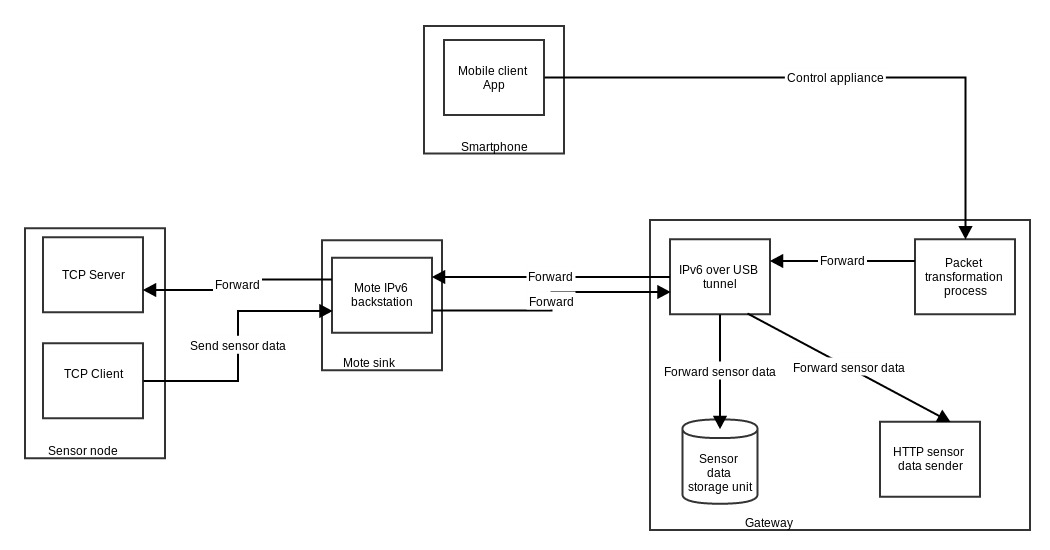
\includegraphics[width=17cm,height=20cm,keepaspectratio]{img/general_architecture.jpg}
\caption{General architecture depicting the main components of the system}
\label{fig:gen_architecture}
\end{figure}
%\clearpage
\paragraph{}
Now that the general architecture has been defined, the question that should be asked is whether all these components operate in the same layer in the \gls{osi} model and if not, in which layer does each of these components reside. As an answer to such a question, figure \ref{fig:layered_view} is here to show in what layer does every component operates.

\begin{figure}[htbp]
\centering
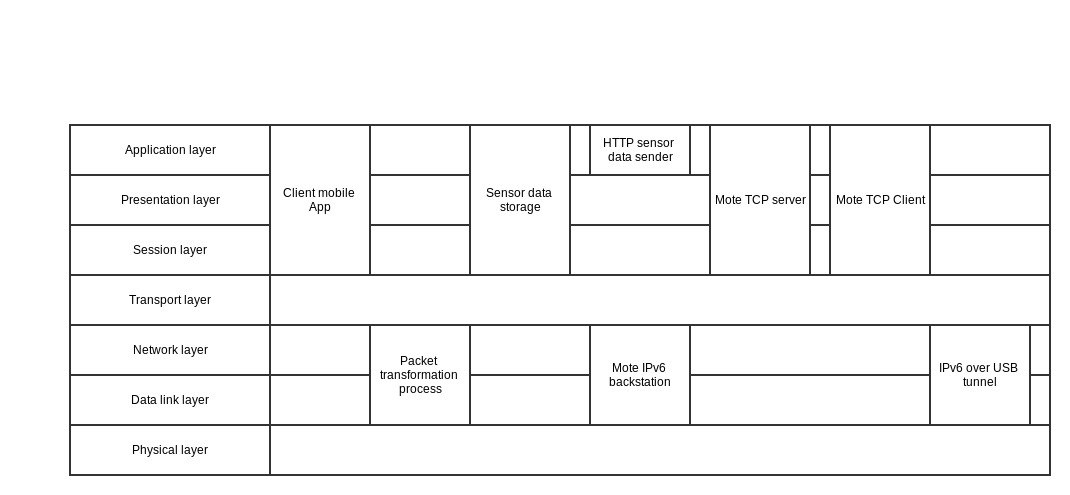
\includegraphics[scale=0.40]{img/layered_view.jpg}
\caption{Layered view showing where every component operates in the \gls{osi} model}
\label{fig:layered_view}
\end{figure}

\paragraph{}
From figure \ref{fig:layered_view}, one can see that there are three components in performing in the data link layer and network layer. The first one is the \gls{ipv4}/\gls{ipv6} gatewaying process whose goal is to hide the communication heterogeneity by sniffing incoming packets, transforming them in order to meet the recipient's communication technology and standards. The second component performing in the data link layer and network is the \gls{ipv6} over USB tunnel; This component is in charge of receiving raw \gls{ipv6} packets and encapsulate them in  USB frames to reach the destination. The third component is deployed in the sink which is the entry and exit point of the \gls{wsn}. This special mote receives \gls{ipv6} packets encapsulated in USB frames that are forwarded to the destination mote using Zigbee.

\paragraph{}
There are four components that operate in the session layer, presentation layer and application layer and are existing in most of the devices needed in the system. The first one is the client mobile App. This component is implements a TCP client and uses most of the services provided by the layers it is operating in. The second component is the sensor data storage which constitutes of a TCP server receiving data from the \gls{wsn}, transforming and storing it in a \gls{rdbms}. The third and fourth components are the Mote TCP client and server that send sensor data and through the TCP client and receive commands using the TCP server. 
\paragraph{}
The only component acting in the application layer exclusively is the HTTP sensor data sender which provides a gateway to other applications that need this data. This component receives data and communicates it to the destination using HTTP. The middle-ware application used HTTP to get sensor data from this system.
\paragraph{}
Now that the general structure of the software system has been established, the hardware structure will be presented and explained further. figure \ref{fig:network_diagram} is a network diagram that shows the hardware components in this system. The \glsreset{wsn}\gls{wsn} appears on the right of the figure. Attached to it the sink that which constitutes and entry and exit point for the \gls{wsn}. This sink is attached to the gateway server through USB a the gateway sees it as a network interface card. In addition, the gateway is equipped with a Wi-Fi interface card that enables it to communicate with the other parts of the system such as the middle-ware and the mobile client, and connect to the Internet.

\begin{figure}[htbp]
\centering
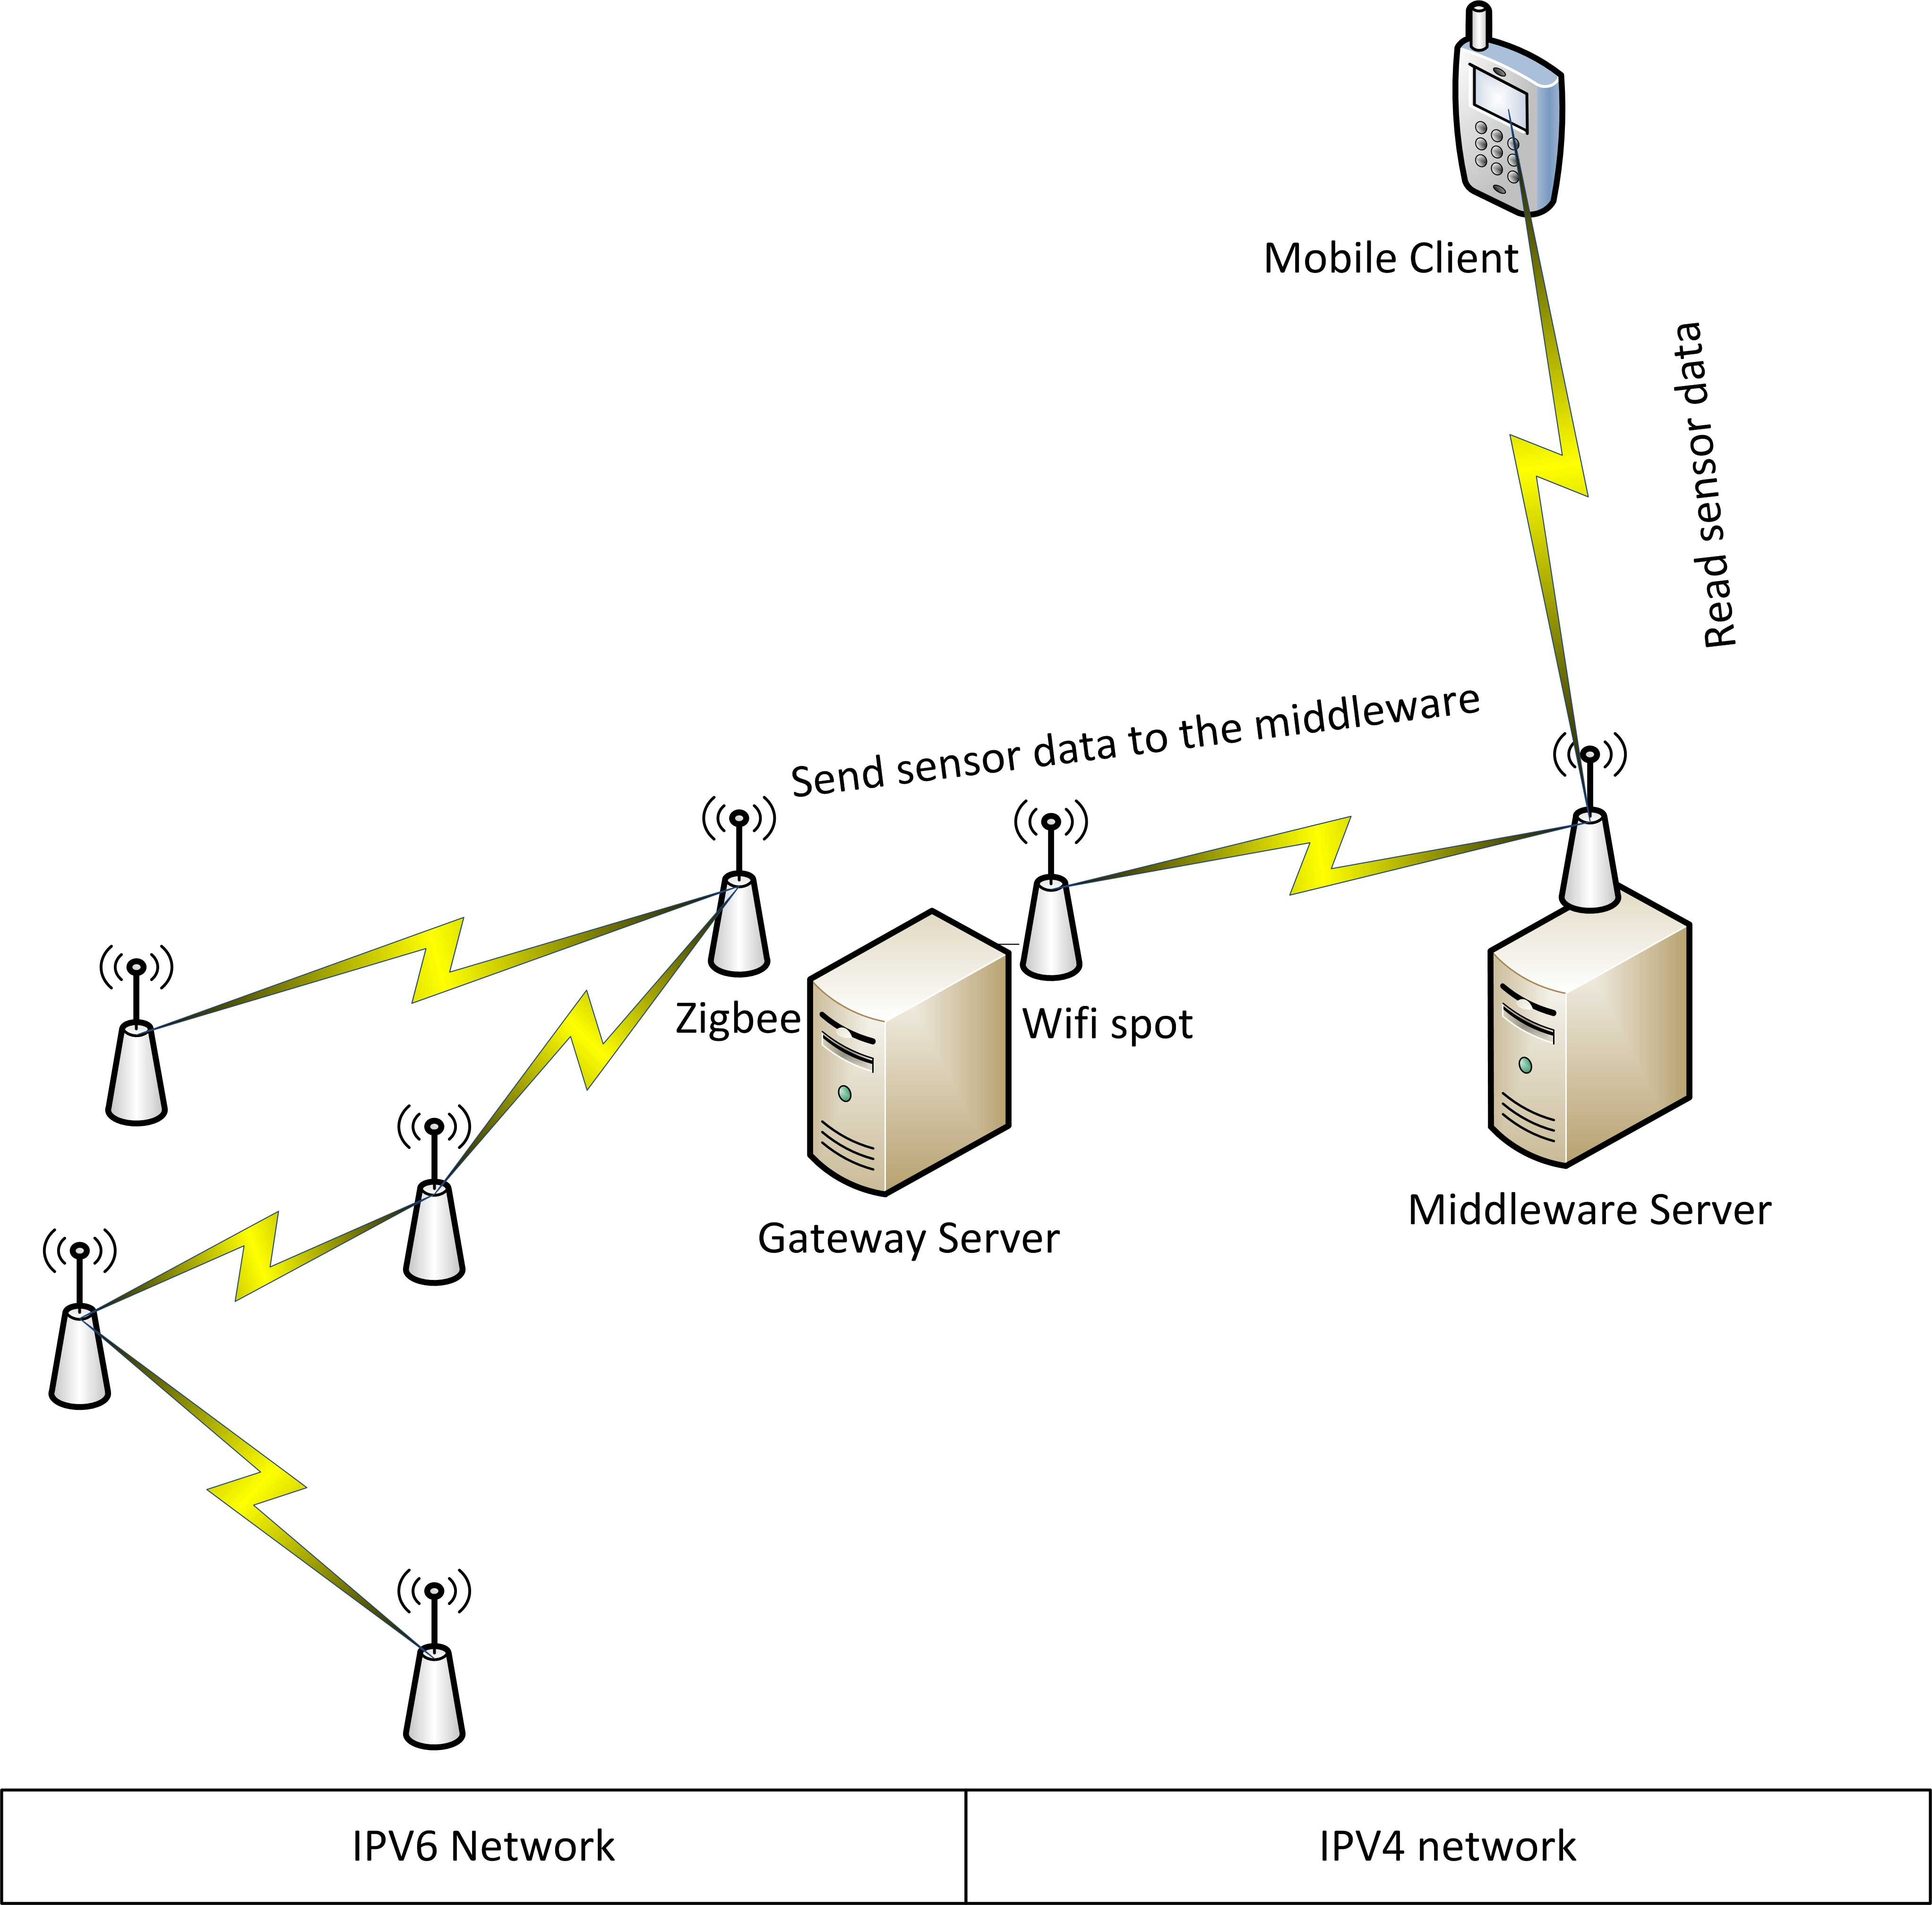
\includegraphics[scale=0.8]{img/network_diagram.jpg}
\caption{Network diagram of the system}
\label{fig:network_diagram}
\end{figure}

\paragraph{}
Now that the network diagram has been established in \ref{fig:network_diagram} where the hardware component are depicted, we need to show where each software component is deployed. In other words, what are the software components that exist on which hardware machine. This is the goal of the matrix appearing in table \ref{table:soft_hard_deployment}. It shows where very software component is deployed. From the table \ref{table:soft_hard_deployment}, it is clear that there are hardware machines that have more than one component deployed and this is also the case for small devices such as sensor nodes within the \gls{wsn}.

\begin{table}
    \begin{tabular}{lllll}
    		  \hline
    Software component - Hardware component & Mote & Mote sink & Gateway & Mobile \\ \hline
    Mote sensor data collection TCP client  & X    & X         & ~       & ~      \\ 
    Mote appliance control TCP server       & X    & X         & ~       & ~      \\
    \gls{ipv4}/\gls{ipv6} Gatewaying Process   & ~    & ~         & X       & ~      \\
    IPv6 over USB tunnel                    & ~    & ~         & X       & ~      \\
    Mote IPv6 back station                   & ~    & X         & ~       & ~      \\
    Sensor data storage process             & ~    & ~         & X       & ~      \\
    HTTP sensor data sender                 & ~    & ~         & X       & ~      \\
    Mobile client                           & ~    & ~         & ~       & X      \\
    \end{tabular}
    \caption{Software-hardware deployment table}
    \label{table:soft_hard_deployment}
\end{table}

\paragraph{}
In the following sections, each software component will be described in more details showing why such a component is crucial and what are the architectural decisions made to become what it is.

\section{Mote Sensor Data Collection-TCP Client}
\paragraph{}
The mote sensor data collection TCP client is a simple \gls{tcp} client deployed in a mote that is equipped with a \gls{ct} attached to an appliance that reads sensory data periodically as shown in figure \ref{fig:current_transformer}. This data needs to be transformed using a set of transformation functions to get the consumption in \gls{wh}. The original value returned is a voltage value in \gls{v} that is then transformed into the current intensity in \gls{a} and with the use of second transformation function, we get the consumption.

\begin{figure}[htbp]
\centering
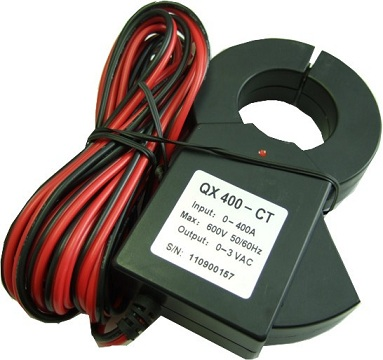
\includegraphics[scale=0.7]{img/ct.jpg}
\caption{Current transformer}
\label{fig:current_transformer}
\end{figure}

\begin{table}
    \begin{tabular}{ll}
    \hline
    slope    & 66.7 \gls{a} \\ \hline
    Constant & 0 \gls{a}    \\ \hline
    \end{tabular}
    \caption{Current Transformer values}
        \label{table:CT_vals}
\end{table}
To transform the initial voltage into the current intensity, we use constant variables provided by the \gls{ct} manufacturer. But these value cannot be taken for granted. To measure them, we conduct an experiment to using the Voltmeter and Ampere meter to measure the slope, $s$, and the function constant, $i_0$, of the intensity transformation function. This function resulted in the following values: 
\begin{itemize}
\item $s = 66.70$
\item $u_0 = 0$
\end{itemize}
Therefore, the first transformation function is: \\
\boldmath{$I = 66.7U_0$} \\
I: Intensity in \glsreset{a}\gls{a} \\
$U_0$: The voltage read from the \gls{ct}

\paragraph{}
Afterwards, we assume the voltage in Moroccan households is 220\gls{v} we get the power using the following function:
\\
\boldmath{$ P = 220I $} \\
P: Power in \gls{w} \\
I: Intensity in \glsreset{a}\gls{a}
\paragraph{}
To get the consumption we use an the sampling rate. The sampling rate is as the number of sensory readings per hour. If one reads sensor data every second, then the sampling rate is 3600 samples per second.
\paragraph{}
To find the consumption, we need to have consecutive sensor readings that we call $P_0$ and $P_1$ and use the following function:
\\
$ C = \cfrac{P_0 + \cfrac{P_1 - P_0}{2}}{S} $ \\
C: Current Consumption in \glsreset{wh}\gls{wh} \\
P: Power sample number 1 in \glsreset{w}\gls{w} \\
P': Power sample number 2 in \glsreset{w}\gls{w} \\
$U_1$: Electrical potential difference or Voltage in households in \glsreset{v}\gls{v} \\
S: Sampling rate \\
The assumption made is that if the power varies between two consecutive samples, the change was linear throughout the interval of time between the two sensory readings.
\paragraph{}
Once the consumption data in hand after this series of transformation, the next thing left to do is to communicate this data. To send it, the mote uses the \gls{tcp} client built on top of the \gls{blip} package that implements the TCP/IP protocol stack. Most important, the system is built in a way that forces all motes to communicate the sensor data gateway services by default, and it will be the gateway's responsibility to manage it (store or communicate it to an external system).

\section{ Mote Appliance Control-TCP server}
\paragraph{}
The mote appliance control \glsreset{tcp}\gls{tcp} server is deployed in all the sensor nodes of the \gls{wsn} including the sink . The goal of this TCP server is be ready to receive commands from external node in the Internet in order to turn On or Off the appliance it oversees. To control an appliance.
\paragraph{}
Figure \ref{fig:appliance_control} depicts the architecture as well as the data flow of the command to turn On/Off an appliance. The TCP server hosted in the mote receives On/Off commands from an external TCP client. The command is then extracted from the IP packet, and based on the command sent, the PIN is identified. Afterward, the command is delegated the MDA320CA that executes it on the chosen PIN by opening (Off) or closing (On) the circuit who is feeding the appliance with electricity.

\begin{figure}[htbp]
\centering
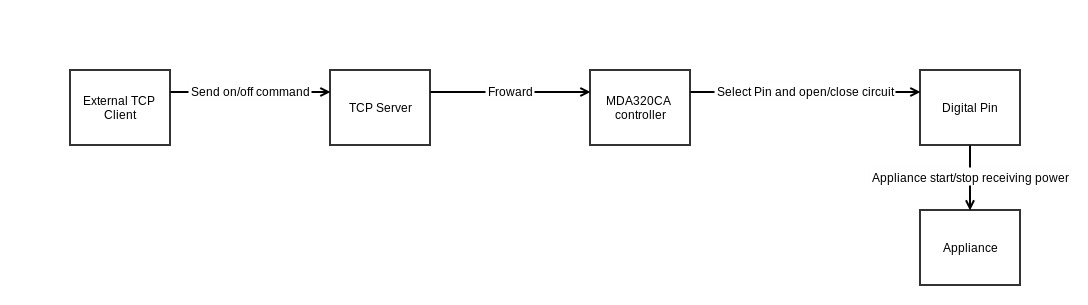
\includegraphics[scale=0.35]{img/appliance_control.jpg}
\caption{TCP Server controlling appliance}
\label{fig:appliance_control}
\end{figure}

\paragraph{}
The mote on itself does not have the necessary hardware capabilities to control an appliance. It needs to be equipped with a Data Acquisition board also known as Extension Board that enable the mote to have more capabilities and therefore the ability to control the power flowing into the appliance. The extension board used in this project is the Crossbow MDA320CA as depicted in figure \ref{fig:mda320ca}. This board has Pins which are electrical inputs and outputs that permit possible to have external analog sensors, digital sensors and also the possibility feeding electricity to the appliance. However, the power supply of the appliances from the mote is not straightforward.
\paragraph{}
To make a mote control the appliance, the mote will govern the supply of electricity by controlling a small circuit that is responsible for pipelining the power flowing to the appliance. In short, the mote is equipped with an extension board to which an electric circuit is attached and whose responsible for the flow of power going to the appliance. Thus, the turn Off command will open the circuit and the appliance will stop getting fed electricity.

\begin{figure}[htbp]
\centering
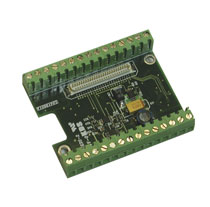
\includegraphics[scale=0.8]{img/mda320.jpg}
\caption{Crossbow MDA320CA Data acquisition board}
\label{fig:mda320ca}
\end{figure}

\section{Mote IPv6 Back station}
\paragraph{} 
This component is deployed only the sink of the \glsreset{wsn}\gls{wsn}. This mote is able to communicate with the sensor nodes using Zigbee and with the gateway using \gls{usb}. The software component deployed in this sink is a packet forwarder. In fact, once it receives an \gls{ipv6} packet that is going outside the \gls{wsn}, it is forwarded through \gls{usb}.
\paragraph{}
The component's goal is to forward packets in and out of the \gls{wsn} while other sensor node do not need to worry about how the packet will be communicated. This mote as part of the components aiming to solve the heterogeneity problem, provides communication transparency.

\section{IPv6 over USB Tunnel}
\paragraph{}
The gateway server machine is equipped with two interface cards: the Wi-Fi and the Zigbee network interface cards. The Zigbee network interface card is of interest in this section. To have a device communicating using Zigbee, one sensor node within the \gls{wsn} was used for this purpose, and the software component implemented in this sensor node is the one described in section 4.6. Indeed, the packet is received through \gls{usb} but not read and recognized as a packet belonging to the TCP/IP protocol stack. To do so, a tunnel was used for the purpose of extracting packets from the \gls{usb} port. In addition, the tunnel was used to forward \gls{ipv6} packets through \gls{usb}.

\section{IPv4/IPv6 Gatewaying Process}
The \gls{ipv4}/\gls{ipv6} Gatewaying Process is one of the components that hides the heterogeneity that exist in the system. This component mainly deals with transforming packets since it extracts the datagram from the packet and create a completely new one that holds the datagram originating from the first one and communicates it. This component is composed of three subcomponents:
\begin{itemize}
\item Packet sniffer
\item Packet transformer
\item Address translator
\end{itemize}
\paragraph{}
Figure \ref{fig:gateway_transformation} depicts the architecture of this subsystem by showing the different subcomponents and their interactions. Moreover, it illustrates the data flow within this subsystem by showing the inputs and outputs of the subsystem.

\begin{figure}[htbp]
\centering
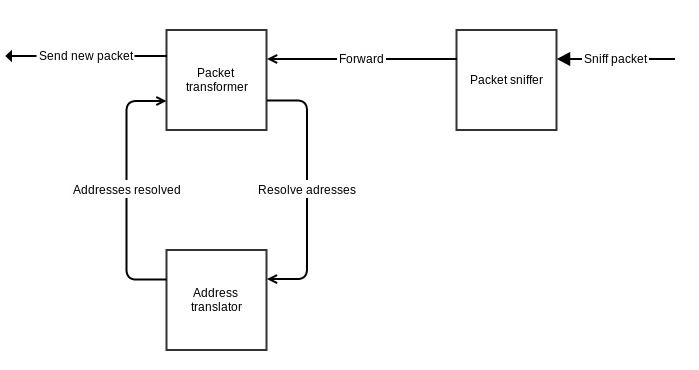
\includegraphics[scale=0.6]{img/packet_transformation.jpg}
\caption{Gateway packet transformation subsystem data flow}
\label{fig:gateway_transformation}
\end{figure}
\paragraph{}
The subsections 4.8.1 to 4.8.3 will detail and explaining the three subcomponents of the system.

\subsection{Packet Sniffer}
\paragraph{}
The packet sniffer subcomponent is the one responsible for sniffing and forwarding the packets to the packet transformer. It does not forward the packets whose recipient is the gateway machine. Specifically, all the packets to be routed by the gateway server are sniffed and forwarded to the packet transformer.
\subsection{Packet Transformer}
\paragraph{}
Once the packet is delegated to the packet transformer, it checks the source of the packet to differentiate between packets incoming from the \gls{wsn} and the packet going to the mote. Concerning the packet not originating from the \gls{wsn}, only those going to \gls{wsn} are processed. But a problem presents itself: 
\underline{The outside world mostly uses \gls{ipv4} whereas the \gls{wsn} uses exclusively \gls{ipv6}}
\paragraph{}

In general, two networks using different network layer technologies cannot communicate despite the fact that \gls{ipv6} is just a new version of the very known \gls{ipv4}, and this is due to the fact that \gls{ipv6} has no backward compatibility with \gls{ipv4}.
\paragraph{Solution}
To solve this problem, we provided all the nodes with both an \gls{ipv4} and \gls{ipv6} address. The nodes have either \gls{ipv4} or \gls{ipv6} addresses, so the one missing is assigned to them virtually. For instance, a sensor node in the \gls{wsn} with a real \gls{ipv6} address equal to FEC0::1 will be assigned a virtual \gls{ipv4} address equal to 192.168.0.1 but he will not be aware of it. Only the Gateway packet transformation component will be aware of it and based on this, we transform the packets and hide the heterogeneity from the components of the system.
\paragraph{}
After the reception of a packet, the Packet Transformer checks whether this component originated from the \gls{wsn} or an external node, and depending on that, it extracts the data from the packet which can be a \gls{tcp} or \gls{udp} datagram. The source and destination addresses are extracted from the packet and translated. Afterwards, a new packet referring to the destination technology used is created by having as a source and destination addresses the translated IP addresses and as payload the \gls{tcp} \gls{udp} datagram extracted from the original packet. Finally, the packet is forwarded to the network.
\subsection{Address Translator}
The address translator is a very specialized subcomponent whose sole goal is to translate addresses from \gls{ipv4} and \gls{ipv6} and vice versa. That is said, this component receives the address to translate and returns the translated one. In fact, the translation function yields a bijective function. that is, for any \gls{ipv4} address there is one and only one \gls{ipv6} address resulting translation and vice versa. This statement compresses a set of statements which are the following:

\begin{itemize}
\item Any address belonging to one technology can be translated to the other technology. This is known as surjectivity.
\item Any address cannot be translated into more than one address from the other technology. This is known as injectivity.
\end{itemize}

\paragraph{}
The gateway packet transformation process is an important component responsible for hiding the heterogeneous nature of the system. It hides most of the heterogeneity in the system and makes communication happen independently of the data link layer or network layer technologies used.

\section{Sensor Data Storage Process}
\paragraph{}
The sensor data storage process is a small component within the system whose goal is to store sensory data. It is perceived by the \gls{wsn} as a TCP server, where sensor nodes get connected to as soon as they boot. The sensor node starts sending packet periodically and whenever the sensor data is received, it is stored into a \gls{rdbms} adopting the schema depicted in figure \ref{fig:erd}.

\begin{figure}[htbp]
\centering
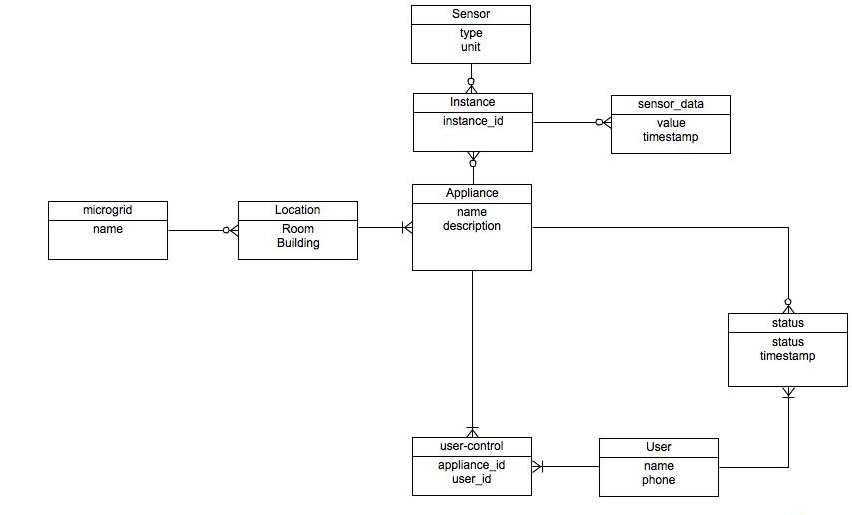
\includegraphics[scale=0.5]{img/smart_grid_db.jpg}
\caption{Entity relationship diagram}
\label{fig:erd}
\end{figure}

\section{HTTP Sensor Data Sender} 
The HTTP sensor data sender is TCP server to which sensor nodes get connected to, and start sending their data periodically. Once the data is received, this component communicates this data to the external node interested in receiving this data. This system relies on the deployment of an HTTP server at the level of external client and sends an HTTP request containing the sensor data received from the \gls{wsn}. 
\paragraph{}
The sensor nodes communicate this data by themselves directly to the external nodes, as this is part of the two-way communication, but for convenience, it was decided that the \gls{wsn} sends its data to the gateway, and it is up to the gateway to communicate it or store it in the \gls{rdbms}.
\section{Mobile Client}
The mobile client is a component of the system but can be perceived as an external world client as it is here to receive sensor data and also send ON/OFF commands to the system.

\chapter{Deployment}
\paragraph{}
In this chapter, the test-bed will be discussed from the implementation point of view. In fact, each component within the system will be given as much details as possible in order for the reader to open the code and understand how it is implemented. Chapter 4 discussed the components from the architectural aspect whereas in this chapter, implementation and technology decisions will be clarified.
\section{Technology Enablers}
The system was built using a set of software and hardware technologies and standards throughout the course of this project to make the test-bed achieve its objectives.
\glsreset{wsn}
\subsection{\gls{wsn}}

\begin{figure}[htbp]
\centering
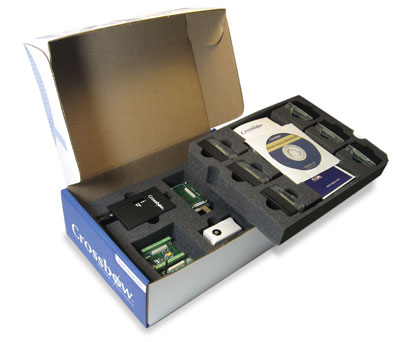
\includegraphics[scale=0.6]{img/crossbow.jpg}
\caption{Crossbow Professional Kit}
\label{fig:crossbow}
\end{figure}

The \gls{wsn} was built using Crossbow professional kit as depicted in figure \ref{fig:crossbow} which counts 7 Micaz sensor nodes of type MPR2600 as shows in figure \ref{fig:micaz}.
\begin{figure}[htbp]
\centering
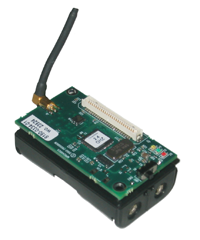
\includegraphics[scale=0.8]{img/micaz.png}
\caption{Crossbow MPR2600 Micaz Mote}
\label{fig:micaz}
\end{figure}

In addition, the motes are supplied with sensor boards of type Crossbow MTS400CA that contain temperature, humidity, barometric pressure, ambient light and infrared light sensors that are used to communicate different types of sensor data to the gateway. This board is shown in figure \ref{fig:mts400}.

\begin{figure}[htbp]
\centering
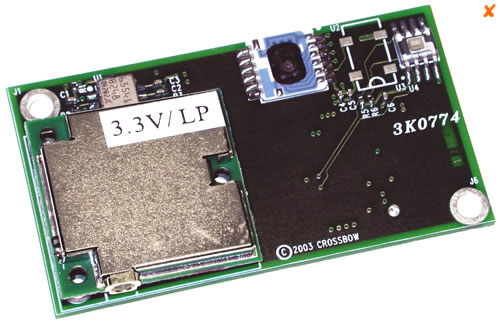
\includegraphics[scale=0.5]{img/mts400ca.jpg}
\caption{Crossbow MTS400CA Sensor Board}
\label{fig:mts400}
\end{figure}
\paragraph{}
The WSN is run using \gls{tinyos} which is one of the most used open source \gls{os} in \glspl{wsn}. Programs are implemented using \gls{nesc} which is the sole programming language used in the \gls{tinyos} environment. This programming language is event-oriented and its syntax is similar to C. In addition, C libraries can be used in \gls{nesc} programs.

\subsection{Gateway}
\paragraph{}
The gateway's hardware machine is Dell Optiplex 9010 running a Linux environment more specifically the Ubuntu 13.04 distribution. The gateway has a set of technologies used to provide numerous services the system relies on. The programming languages used in the components deployed in this machine are C and \gls{j2se}. Netfilter is also used to drop incoming packets. Concerning the storage of sensor data, MySQl is the \gls{rdbms} used.

\subsection{Mobile Client}
\paragraph{}
The mobile used is a smart phone running Android 2.3. The application developed is using \gls{j2se} and PHP for database connectivity.

\section{Mote TCP Client And TCP Server}
\paragraph{}
Section 4.4 and 4.5 were dedicated to explain the TCP Client and TCP server separately. In this section, one section will explain both of them because from the implementation point of view,  both are implemented in the \gls{tinyos} program.
\paragraph{}
A typical \gls{tinyos} program has two parts: the components definition part and the module part. In the components definition part, the main components that will be used are declared. These components refer to already-implemented modules whose functionalities will be called in the in-development module. In the module part, we define the interfaces we will be using and those we will be providing. Back to definitions part, after defining components that will be used, we then link the interfaces needed in the module to the components providing those interfaces. This step is called wiring \cite{ref14}.
\paragraph{}
The components needed in this program are the following:
\begin{itemize}
\item MainC: provides the essential functionalities such as the initialization and closing of the program.
\item LedsC: provides access to the leds existing in the mote
\item Taos2550C: is a light sensor component that enable to read data
\item TimerMillic: A Timer that will be used for sampling
\item TCPSocket as client: Is the TCP client
\item TCPSocket as Server: Is the TCP server
\end{itemize}
In the modules part we define the components that will be used which are the following:
\begin{itemize}
\item Boot: This is the interface that provides main functions of booting and closing
\item TCP as server: The main interface for TCP
\item TCP as client: The main interface for TCP
\item Leds: The interface to access the leds
\item timer as sensingTimer: The interface to program and use the timer
\item Read as Sensor: The interface to talk with the sensor
\end{itemize}
The interfaces one uses have some functions that are not implemented and should be written in the module. The following part discusses the main functions:
\paragraph{After boot of the mote}
The first thing that is done after the mote is booted is to initialize the TCP client and server. The Client is binded to a random port. The TCP server is binded to port 7. The client gets connected to the Data store in the gateway by providing the \gls{ipv6} address of the gateway and port number of the server. Afterwards, the timer is set to be triggered every 10 seconds which means that the sampling rate will be 360 sensor readings per hour. 
\paragraph{TCP Server data received}
Once the data is received from a client, it assumes that there are two data items separated by a space. The first item refers to the led number(1,2,3) and the second refers to the command 0 meaning turn Off and 1 means turn On. The string is tokenized and the data items are extracted and the command is executed accordingly.
\paragraph{Timer fired}
Once the timer is fired, it is time to read sensor data from the sensor. The command to read from the sensor is called reads data and once the data is read the event "read done" is triggered.
\paragraph{Read done}
Once the data is read and ready, the next thing is to transform it and then send it. Concerning the transformation, a series of equations are applied as seen in section 4.4 which builds the data value from the original value. A message is created containing two values: the mote NODE\_ID which is the identifier of the mote predefined in the installation of the program in the mote and the sensor data value. These two values are separated by a space, encapsulated within a \gls{tcp} datagram and sent. The NODE\_ID is not necessary to identify the mote because the mote can be identified using its \gls{ipv6} address.
\paragraph{}
During the installation of the software, the \glsreset{blip}\gls{blip} package should specified as the program depends on it. \gls{blip} provides the TCP/IP protocol stack that implements \gls{6lowpan} standard by \gls{ietf}. In  the installation, the NODE\_ID is specified. If NODE\_ID is 1, this will make the mote have an \gls{ipv6} of FEC0::1, as the NODE\_ID is appended to the predefined prefix of \gls{wsn} during the installation.
\section{Mote IPv6 Back station}
\paragraph{}
This component is included in the \gls{blip} software package. It is a \gls{tinyos} program whose goal is to forward packets back and forth between the \gls{wsn} and the external networks. This mote is connected to the \gls{wsn} using Zigbee, and to the outside world using \gls{usb}. This mote's \gls{ipv6} address is FEC0::64. It receives \gls{ipv6} packets which are encapsulated in \gls{usb} frames, extracts them and encapsulates them in a Zigbee frame and vice versa.
\paragraph{}
During the installation of this \gls{tinyos} program into the sink, one should make sure that it is installed in the mote sink device because \gls{usb} is crucial. The \gls{ipv6} address does not need to be provided because it is already predefined in the program configuration file.

\section{IPv6 over USB Tunnel}
\paragraph{}
This program is installed in the gateway server machine. The sink gets connected to the gateway using \gls{usb}, the gateway will recognize it as a network interface card that uses \gls{ipv6} as a network technology. Moreover, this component is part of the \gls{blip} software package which the network interface card module and starts extracting incoming \gls{ipv6} packets from the \gls{usb} frames and encapsulates outgoing \gls{ipv6} into \gls{usb} frames.
\paragraph{}
The installation and initialization of this component will be detailed in appendix A.
\section{IPv4/IPv6 Gatewaying Process}
\paragraph{}
This component is in charge of hiding the heterogeneity of the system from the rest of the components of the system and also the outside world. It does so by intercepting all the packets and transforms the ones of interest to meet the standards used by the recipient.
\paragraph{}
To make use of this process, there is an initial configuration that should be performed on all the components of the system in order for the system to work (explained in Appendix A). The gateway has two network interface cards: the Wi-Fi interface and the Zigbee interface provided through the tunnel. The first one is using \gls{ipv4} whereas the second is using \gls{ipv6}.
\paragraph{}
The program has three subcomponents as seen in section 4.8. The three components are the following:
\begin{itemize}
\item Packet sniffer
\item Packet transformer
\item Address translator
\end{itemize}
The following subsections will discuss each of these subcomponent separately from the implementation point of view.

\subsection{Packet sniffer}
\paragraph{}
The packet sniffer is the one in charge of sniffing packets from both network interface cards, as Raw Frames. The code snippet shows the functions called to sniff the packets. We make use of the Raw Socket library that enables us to sniff the Data Link Layer frames before dropping them using Netfilter.
The main reason behind dropping the packets is when packets are received by a station who has an empty routing table, this station will automatically send ICMP REDIRECT TO HOST messages to the sender meaning that the route chosen by the sender is not the appropriate one, therefore the sender will stop sending packets to that station.

\begin{lstlisting}
sockfd = socket( PF_PACKET, SOCK_PACKET , htons(ETH_P_ALL));
if (sockfd < 0)
	exit(1);
	
while(1)
{
	data_size = recvfrom(sockfd,buf,10000,0
		,(struct sockaddr *)&cliaddr,&clilen);
}

\end{lstlisting}
\paragraph{}
The first line of code initializes the Raw Socket, we define the type, scope and name space of the packets to be sniffed. This will return a file descriptor that will allow us to call the socket. Afterwards, we start reading packets in an infinite loop.

\paragraph{}
After sniffing a packet, we must check if it is an \gls{ipv4} or an \gls{ipv6} packet. The problem is that when reading from the Wi-Fi interface card, we get the second layer frame where the network packet is encapsulated, but the Zigbee Tunnel only gives the third layer raw \gls{ipv6} packet. Once a packet is read, one cannot identify the interface card providing it, and therefore a partial solution is found. We cast the packet to Wi-Fi frame and check next header's protocol number. There are two solutions: 0 referring to \gls{ipv6} and 8 referring to \gls{ipv4}.
If we get zero, the whole data should be casted to the \gls{ipv6} data structure whereas if it is 8, we should move the pointer forward to omit the Wi-Fi header and cast the following part to the \gls{ipv4} data structure.
\paragraph{}
In each of those conditions, we only select the TCP datagrams, and this is why we check if the next header in the IP structure is equal to 6. After that, we move the pointer to ignore the IP header and only keep the TCP datagram that will have to be sent in a the newly created packet. Depending on the network technology of the sniffed packet, we should build a new packet with the technology that is recognized by the recipient.

\begin{lstlisting}
if(header->h_proto == 0) 
{
	if(ip6_hdr->ip6_nxt == 6)
	{
			buf += IP6_HDRLEN;
			... 			
			sendIPV4Packet(..)
	}
}
else if(header->h_proto == 8)
{
	if(ip_hdr->protocol == 6)
	{
		buf += (sizeof(struct ethhdr)+ IP4_HDRLEN);		
		...
		sendIPV6Packet(...)
	}
}
\end{lstlisting}

\subsection{Packet transformer}
\paragraph{}
The packet transformer subcomponent is in charge of building two types of packets: \gls{ipv4} and \gls{ipv6} packets. As stated in section 4.8, all devices in this system have both an \gls{ipv4} and \gls{ipv6} address, where one of them is only recognized at the gateway. The \gls{wsn} exclusively supports \gls{ipv6}. Therefore, the sensor nodes cannot be addressed without \gls{ipv6}, but any device not using \gls{ipv6} may communicate with them by using their virtual \gls{ipv4} addresses. Once the packet reaches the gateway, it is transformed in order for the data carried to be delivered. Therefore, the packet will have instead of \gls{ipv4} source and destination addresses, \gls{ipv6} addresses that will be translated using the Address translator subcomponent.
\paragraph{}
This subcomponent is based on two important functions:
\begin{itemize}
\item sendIPv6Packet(..)
\item sendIPv4Packet(..)
\end{itemize}
\paragraph{}
The idea is the same, except that each technology has its own details such as filling different packet fields and computing the checksum. Another difference is when creating the \gls{ipv4} packet, one should also create the Wi-Fi frame otherwise it won't be able to be sent through the Wi-Fi network interface card. But when building \gls{ipv6} packet one should only send the packet and the tunnel will take care of encapsulating it into a \gls{usb} frame.
The sendIPv6Packet() function receives the data to be sent, which is a \gls{tcp} datagram, along with the size of the datagram, and the translated source and destination addresses. Afterwards, the transformer creates the packet appends to it the datagram, fills the source and destination addresses and create a Socket linked to the corresponding interface card and sends the packet.
\begin{lstlisting}
int sendIPV6Packet(char* buffer,int size,char *src ,char *dest)
{
	//CREATE PACKET WITH ALL ITS DETAILS
	...
	memcpy (frame + IP6_HDRLEN, buffer, size);
	sd = socket (PF_PACKET, SOCK_RAW, htons (ETH_P_ALL))) < 0);
	sendto (sd, rame, length...);
}
\end{lstlisting}

\subsection{Address translator}
\paragraph{}
The address translator is the subcomponent that assigns \gls{ipv4} and \gls{ipv6} to all devices in this system. For instance, sensor nodes in the \gls{wsn} have \gls{ipv6} addresses but this subcomponent assigns \gls{ipv4} addresses to them.
\paragraph{}
To do so, the translation algorithm is purely bijective. That is said, any \gls{ipv4} is translated to one and only one \gls{ipv6} and vice versa. For a mobile client with \gls{ipv4} address of 10.50.1.50 to communicate with a mote whose \gls{ipv6} address is FEC0::1, the mobile client should be aware of the mote's translated \gls{ipv4} address which is 192.168.0.1. Once the packet is received, the source and destination \gls{ipv4} addresses are translated to \gls{ipv6} making the source address equal to 0A32::0132 and the destination FEC0::1. The \gls{ipv6} packet is created and reaches the destination which is the sensor node. Once the response is going back, the scenario is similar.
\paragraph{}
The translation algorithm has been tested extensively to make sure it is bijective, and that any address can be translated to one and no more and than one address. When configuring the system, one should make sure that there are no two devices that have the same address, real or virtual. Any \gls{ipv6} and \gls{ipv4} address should be unique throughout the whole system. The \gls{wsn} should be granted an interval of \gls{ipv4} addresses to make sure that no one besides the \gls{wsn} has those addresses.


\chapter{Findings}
\paragraph{}
The system was built to monitor and control home appliances, and to also provide an infrastructure for future platforms to be integrated in this system. An example of infrastructures that can be the integrated is the \glsreset{dr}\gls{dr}. To build overlying system's, one should make sure that the system achieves a performance level that one can count on. The purpose of this chapter is to measure the performance of the system. It is done by conducting two experiments which will help us gather data, and based on that, an interpretation of this data will be done to verify if the system shows an acceptable level of performance.
\section{Experimentations}
\paragraph{}
To measure the performance of the system, two experiment were conducted where the goal is to quantify the performance of the system. There is an architectural decision madein \gls{6lowpan}, and we would like to see if it add more performance to the system. The architectural decision is the following: There is more priority given to routed packet that the processed ones. As a result, this clearly pushes us to think that the delay of the system will not follow the same growth trend as the network traffic.
\paragraph{Experiment 1:}
We start with one mote in the \gls{wsn} that will be interacting with the outside world. We then start sending ping command periodically (once every 1 second) and record the delay and the jitter. Once every two minutes, we will add another mote to the \gls{wsn} and continue pinging the same mote. We keep adding motes every 2 minutes until we reach 6 motes which is the maximum number of motes available. This will enable us to collect data about the mote delay and jitter as we add more traffic to the system.
\paragraph{Experiment 2: }
The second experience is meant to measure the time it takes to transform the packet. In other words, measure the extra delay and jitter when having the Gateway Transformation Process as part of the system. The timer starts before the sniffing of the packet and ends right after the packet is transformed and communicated.
We believe that this transformation adds delay, but we are hoping that this extra delay is not significant enough to affect the whole system.
\section{Data Gathering and Analysis}
\paragraph{}
After both experiments were conducted, we collected a significant amount of data that was used to measure the performance. In addition, we analyze and interpret the results to make judgments about the overall performance of the system.
\subsection{Experiment 1}
\paragraph{}
In the first experiment, the same mote was pinged once every second and we added new motes to the system every two minutes. The experiment as a whole took 12 minutes or 720 pings. Table \ref{table:exp1} shows the result of the experiment.

\begin{table}[htbp]
    \begin{tabular}{lll}
    \hline
    number of motes & Delay (ms) & Jitter (ms) \\\hline
    1               & 87.5         & 1.2         \\ 
    2               & 88.1         & 2.0         \\
    3               & 88.3        & 2.7         \\
    4               & 88.8         & 3.1         \\
    5               & 90.0         & 3.3         \\
    6               & 89.5         & 3.5         \\
    \end{tabular}
    \caption{Experiment 1 delay and jitter}
    \label{table:exp1}
\end{table}
\paragraph{}
For each row in the table, the average delay is computed over the pings performed in the 2 minutes interval or the 120 pings gathered. The jitter is also computed similarly as the average variation from the mean delay in that 2 minutes interval. The result is displayed in the table \ref{table:exp1}. 
\paragraph{}
The data collected shows even though the delay in the \gls{wsn} is high, 
 nothing can be done about that because when the traffic in the \gls{wsn} is low, the delay is still high and this has to do with the computational time taken by the TCP/IP protocol protocol stack provided by \gls{blip} using that implements \gls{6lowpan}. To reduce the delay, one should probably rethink the design of the \gls{blip} and investigate ways to reduce processing time.
 
 \begin{figure}[htbp]
 \centering
 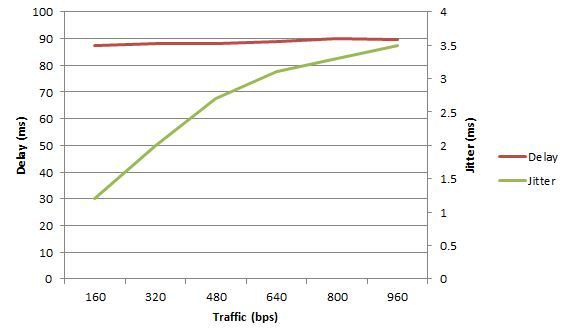
\includegraphics[scale=1]{img/delay_jitter.JPG}
 \caption{Delay and jitter evolution by Bandwidth}
 \label{fig:delay_jitter}
 \end{figure}
 
 \paragraph{}
 The good news in experiment 1 is that the priority of packets brings benefit to the network. Even though the traffic grows exponentially, the average delay stays constant. However, the jitter follows the traffic's trend, but still the average delay shows good results. 
 
\subsection{Experiment 2}
\paragraph{}
The second experiment's goal is to measure the contribution of the Gateway Packet transformation process to the overall communication delay. The results gathered reflect the average delay and jitter computed over the elapsed time starting from the sniffing of the packet to the transformation and sending to the recipient. Table \ref{table:exp2} shows the result that was collected from this experiment as it was done on 200 packets that were sniffed and transformed by the system.

\begin{table}[htbp]
    \begin{tabular}{ll}
    \hline
    Delay (ms) & Jitter (ms) \\ \hline
    0.1        & 0.0         \\ 
    \end{tabular}
    \caption{Experiment 2 delay and jitter}
        \label{table:exp2}
\end{table}
\paragraph{}
The transformation process's elapsed time is measured in milliseconds and from table \ref{table:exp2}, one can see that the average delay is on average 0.1 milliseconds whereas the jitter is around 0 milliseconds meaning that the process's time varies between a few nanoseconds to at most 150 nanoseconds. Depending on the machine's load. The distribution of the delay frequency is shown the histogram depicted in figure \ref{fig:histogram}. From this figure one can conclude that the delay is normally distributed
\begin{figure}[htbp]
 \centering
 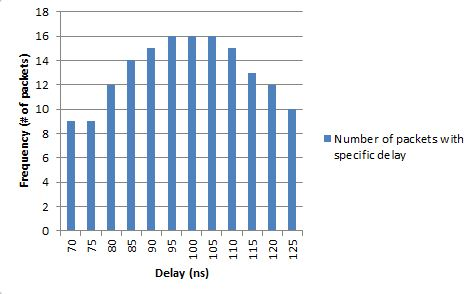
\includegraphics[scale=0.9]{img/histogram.JPG}
 \caption{Delay frequency histogram}
 \label{fig:histogram}
 \end{figure}
\paragraph{}
 The Packet transformation process is a component that shows excellent results. Before conducting experiment 2, we were persuaded that there will be additional delay originating from this process and it could be responsible for the high delay seen in experiment 1. However, the results show otherwise and that the component is not to be put responsible for such an important delay seen in experiment 1.

\chapter{Conclusion}
\paragraph{}
This project enabled us to create an infrastructure that would be part of the \glsreset{iot}\gls{iot} and move towards having the smart home system's integrated within the Smart Grid. At this stage and counting solely on this work, one cannot clearly see the integration of smart home systems within the \gls{iot}, but this is an infrastructure that provides two main services which are the establishment of the two-way communication between the smart home devices and the outside world, and the heterogeneity handler. The two-way communication enables the \glsreset{wsn}\gls{wsn} to monitor home appliances and send sensor data to a repository and this last can be used to simulate a real world \gls{ami}. The second direction in this communication gives the ability for clients to control appliances by turning them On or Off.
\paragraph{}
The second contribution of this work is the smart management of the heterogeneity. The communication from the mote to the mobile client uses a set of technologies and the journey of a simple \gls{tcp} datagram goes through many different Data Link Layer standards and different Network technologies. Starting from the mote sending sensor data, The TCP data is encapsulated into an \gls{ipv6} packet that is encapsulated into a Zigbee frame. Afterward, the packet is extracted from the Zigbee frame and encapsulated into a \gls{usb} frame. Once it arrives to the gateway, the \gls{tcp} datagram is extracted from the \gls{ipv6} which is extracted from the \gls{usb} frame and encapsulated in an \gls{ipv4} packet that is encapsulated into a Wi-Fi frame and sent until it reaches the mobile. That is said, it clear that the system is heterogeneous and making this heterogeneity transparent was a contribution of this work.
\paragraph{}
The \glsreset{wsn}\gls{wsn} was built using the very recent \gls{6lowpan} whose goal is to provide the TCP/IP protocol stack to the smallest devices. The \gls{wsn} is autonomous in the sense that it can monitor the home appliances independently and indefinitely. 
\paragraph{}
All in all, this project as a big picture creates a test-bed providing the main components of a smart home management with an intelligent \gls{wsn}, a robust and powerful middle ware application that is able to use the sensory data and use it to control the home's appliances and a mobile application able to provide the users with remote monitoring and control of their smart homes. This was possible by making the system part of the \glsreset{iot}\gls{iot}.
\chapter{Future Work}
\paragraph{}
The goal of this thesis was to establish the infrastructure for integrating smart home within \glsreset{sg}\gls{sg} and make it part of the \glsreset{iot}\gls{iot}. This project enabled the deployment of the two-way communication as an infrastructure that can be used to build the \glsreset{dr}\gls{dr}. \gls{dr} is one of the most discussed topics in Smart Grids. It enables the utility and households to communicate with a set of services that any of them may request from the other. The current state of the art does not incorporate this communication interface in smart home systems \cite{ref15}. But as there is a need for this communication, \gls{dr} will have to be implemented as part of the smart home package.
\paragraph{}
Demand response integration is a future work for this study. \gls{dr} includes a set of services that have to be implemented in the smart home packages. In \gls{dr}, the consumer has the possibility to ask the utility about the instantaneous price quote for electricity. The consumer when in need of high priority in energy, may ask the utility to guarantee the delivery of a certain quantity of electricity. Of course this comes with a cost, but this agreement is part of the \gls{dr} and should be implemented at the level of smart home systems. Consumers can also help utilities at difficult times. For instance, when the utility cannot provide enough energy at peak times, the utility may ask some consumers to reduce their consumption and as a result be billed a reduced cost for the electricity that is consumed. In general, the smart home aims to reduce energy consumption and as the utility needs to reduce its energy production in peak hours, the \gls{dr} will help the utility ask the smart homes to reduce their consumption.
\paragraph{}
As this project aims to integrate the smart home devices within the \glsreset{iot}\gls{iot}, \glsreset{rfid}\gls{rfid} must be part of this system as a future work. The \gls{rfid} is a building block within the \gls{iot} and will equip the devices with a low-power radio identification mechanism hat will give more flexibility to the system. therefore, the external systems may be able to recognize uniquely each device in the \gls{iot} without counting primarily on their \gls{ipv6} address, which may change from time to time.
\paragraph{}
This system provides near real-time sensory data that is not exploited intelligently. The only use of this data is to enable users to monitor their home consumption. As far as the system is concerned, one must more intelligently exploit this data that can be used by smart algorithms to automatically and autonomously reduce the household's energy consumption. Such algorithms can be based on machine learning and data mining techniques making it a cross disciplinary project aiming to reduce the consumption of households without reducing the utility of users. In other words, building algorithms that will reduce consumption of households while the user is not noticing change.
\paragraph{}
Before building new services on top of this system, one should test different aspects of the system. In this study, the only thing that was tested, measured and quantified was the performance of the system which gave good results about the system's overall performance. As a future work, one should test different aspects of the system such as the reliability and availability of the system. More experiments should be conducted to see how well the system acts in high traffic networks and how good could it support new overlying systems such as \gls{dr}.
\paragraph{}
The system provides different services, but there is no authentication or authorization involved to access the system. In fact, any user knowing the mote's \gls{ipv6} address can control it because there is no existing party or component that controls the flow of information. As a future work, the system should have a third party component whose goal is to make the system secure.

\renewcommand{\bibname}{Index}
\bibliographystyle{IEEEtran} 
\bibliography{IEEEabrv,myrefs}


%\backmatter
\begin{appendices}
\chapter{System Installation}
\section{Hardware needed}
In order for the user to install the system, one should dedicate a computer to host the different services of the system. The crossbow professional kit is a necessity and a router must be available to connect the different components through Wi-Fi. A smart phone or a separate computer with Android emulator may de used.

\section{Software installation}

\subsection{Operating system}
The machine should run Linux Ubuntu distribution (11.10 or more recent). You way use Windows as long as you Install a Virtual machine such as Cygwin for instance.
\subsection{TinyOs Installation}
\begin{enumerate}
\item Execute: sudo gedit /etc/apt/source.list
\item Add to the opened file: deb http://hinrg.cs.jhu.edu/tinyos hardy main
\item sudo apt-get update 
\item sudo apt-get install tinyos-2.1.1
\item sudo gedit ~/.bashrc
\item add the following line: \\
export TOSDIR=\$TOSROOT/tos \\
export CLASSPATH=\$TOSROOT/support/sdk/java/tinyos.jar:.\$CLASSPATH \\
export MAKERULES=\$TOSROOT/support/make/Makerules \\
export PATH=/opt/msp430/bin:\$PATH \\
source /opt/tinyos-2.1.1/tinyos.sh \\

\item sudo chmod 777 \$TOSROOT
\end{enumerate}

\subsection{Configuring \gls{blip}}
\glsreset{blip}\gls{blip} should be compiled before being used. To do so, follow these instructions:
\begin{enumerate}
\item cd \$TOSROOT/support/sdk/c/sf \\
./bootstrap \\
./configure \\
make 
\item cd \$TOSROOT/support/sdk/c/blip \\
./bootstrap.sh \\
./configure \\
make 
\end{enumerate}

\subsection{Install Software in Motes}
The first thing to do is to install the backstation within the Mote sink (the mote with the \gls{usb} IO) To install it we do the following:
\begin{enumerate}
\item Plug the mote and type the command dmesg to see what \gls{usb} ID was assigned to it. It will generally be USB0.
\item cd \$TOSROOT/apps/IPBaseStation
\item make micaz blip install  mib520, /dev/ttyUSB0
\end{enumerate}
The backstation is now installed. We will now install the Mote TCP Client and Server in each sensor node. To do it, we should first download the code from the SVN repository.
\begin{enumerate}
\item Make sure you have SVN by typing svn --version
\item If you do not have SVN type sudo apt-get install subversion
\item download the file:
\item cd
\item svn checkout http://grid-aui-tinyos.googlecode.com/svn/trunk/ grid-aui-tinyos
\item cd grid-aui-tinyos//programming/TCPEcho
\end{enumerate}
Now take the MIB520 programming card, plug it and type dmesg to see where it plugged. lets call the location *USB. Now plug each mote in the MIB520 card and for each plugged mote do the following:

\begin{enumerate}
\item  make micaz blip install.*NUM mib520,/dev/tty*USB
\item make clean
\end{enumerate}
Note that *NUM refers to the NODE\_ID. For the first mote choose 1, for the second choose 2...

\subsection{Install Packet Transformation process}
To install this component, you must do the following:
\begin{enumerate}
\item Make sure you have CMake, type sudo apt-get install cmake
\item cd
\item grid-aui-tinyos//programming/netfiltering
\item cmake CMakeLists.txt
\item make
\end{enumerate}

\subsection{Install Gateway Sensor Data TCP Server}
To install the server you must do the following:
\begin{enumerate}
\item cd
\item grid-aui-tinyos//programming/GatewayServer/src
\item make
\end{enumerate}

\chapter{Run the System}
There is a set of instructions to follow in order as some of the components must be alive only when others are already alive. To run the system, do the following:
\begin{enumerate}
\item To turn on the Tunnel do the following
\subitem cd \$TOSROOT/support/sdk/c/blip/ 
\subitem sudo driver/ip-driver /dev/ttyUSB0 micaz. \\
 You must check that the mote sink is attached to USB0 by using dmesg, if not change it accordingly. After that, you should have an output that looks similar to the figure \ref{fig:tunnel_output}

\begin{figure}[htbp]
\centering
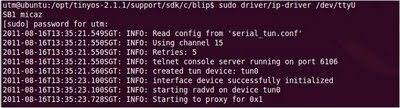
\includegraphics[scale=0.9]{img/tunnel_output.jpg}
\caption{IPv6 over USB tunnel execution output}
\label{fig:tunnel_output}
\end{figure}

\item To Run the Gateway Sensor Data TCP server do the following:
\subitem cd
\subitem cd grid-aui-tinyos/programming/GatewayServer/src
\subitem java Server

\item To Enable IP forwarding do the following:
\subitem sudo bash
\subitem echo 1 \textgreater /proc/sys/net/ipv4/ip\_forward
\subitem exit

\item  To drop all incoming packets: sudo iptables -P INPUT DROP
\item To disable ICPMP REDIRECT TO HOST:
\subitem sudo bash
\subitem /sbin/sysctl -w net.ipv4.conf.all.accept\_redirects=0
\subitem /sbin/sysctl -w net.ipv4.conf.all.send\_redirects=0
\subitem /sbin/sysctl -w net.ipv6.conf.all.accept\_redirects=0
\subitem /sbin/sysctl -w net.ipv6.conf.all.send\_redirects=0
\subitem exit

\item Run the Packet transformation process
\subitem cd
\subitem cd grid-aui-tinyos/programming/netfiltering
\subitem sudo my\_sniffer

\item Turn on the wireless sensor nodes one by one
\end{enumerate}

\paragraph{}
You should be able to get sensor data periodically. The mobile client access for turning On and Off will be explained in the Appendix C.
\end{appendices}

\end{document}